% Presentation for LaTeX introduction
\documentclass[t]{beamer}
\usetheme[cabin,darktitle]{UniversityOfManchester}

% Document properties
\title{An Introduction to \LaTeX{}}
\author{Andrew Mundy}

% Code formatting
\usepackage{sourcecodepro}
\usepackage{minted}
\setminted[bash]{
  style=tango,
  bgcolor=black!10!white,
}
\setminted[tex]{
  style=tango,
  bgcolor=black!5!white,
}

% Mathematics
\usepackage{mathtools}
\usepackage{commath}
\usepackage{siunitx}

% Nice table formatting
\usepackage{booktabs}
\usepackage{multirow}

\begin{document}

\maketitle

\begin{frame}{Document Classes}
  \begin{description}
    \item[acmsmall] Some ACM publications
    \item[article] Generic articles
    \item[beamer] Presentations (this is one)
    \item[book] Generic books
    \item[ieeetran] IEEE publications
    \item[report] Like \texttt{book} but with commands for abstracts (think thesis\ldots)
  \end{description}
\end{frame}

\begin{frame}{Text input}
  \begin{itemize}
    \item \mintinline{tex}{``Hello, world''} for ``Hello, world''
    \item \mintinline{tex}{`Hello, world'} for `Hello, world'
    \item \mintinline{tex}{--} for --
    \item \mintinline{tex}{\%} for \%
    \item \mintinline{tex}{\ldots} for \ldots
    \item \mintinline{tex}{\textbackslash} for \textbackslash
    \item \mintinline{tex}{~} for non-breaking spaces, more later
  \end{itemize}
\end{frame}

\begin{frame}{List styles}
  \begin{description}
    \item[\texttt{itemize}] Standard bullet points
    \item[\texttt{enumerate}] Numbered/lettered points
    \item[\texttt{description}] Description list (this is one)
  \end{description}
\end{frame}

\begin{frame}{Font formatting}
  \begin{itemize}
    \item \mintinline{tex}{\textbf{Hello}} -- \textbf{Hello}
    \item \mintinline{tex}{\textit{Hello}} -- \textit{Hello}
    \item \mintinline{tex}{\textsc{Hello}} -- \textsc{Hello}
    \item \mintinline{tex}{\texttt{Hello}} -- \texttt{Hello}
  \end{itemize}
\end{frame}

\begin{frame}{Document Structure}
  \begin{itemize}
    \item \mintinline{tex}{\part{Part title}}
    \item \mintinline{tex}{\chapter{Chapter title}}
    \item \mintinline{tex}{\section{Section title}}
    \item \mintinline{tex}{\subsection{Subsection title}}
    \item \mintinline{tex}{\subsubsection{...}}
    \item \mintinline{tex}{\paragraph{...}}
    \item \mintinline{tex}{\subparagraph{...}}
  \end{itemize}
\end{frame}

\begin{frame}[fragile]{Labels and Cross-Referencing}
  Create labels with \mintinline{tex}{\label{label-name}} command.
  \vfill
  For example:
  \begin{minted}{tex}
\section{A section to refer to later}
\label{sec:chapter-name/section-name}
  \end{minted}
  \vfill
  Then I can refer to the section with \mintinline{tex}{\ref{...}}
  \vfill
  For example:
  \begin{minted}{tex}
As we saw in
section~\label{sec:chapter-name/section-name}
  \end{minted}
\end{frame}

\begin{frame}[fragile, plain]{Figures and Floats}
  With the \texttt{graphicx} package imported.

  \begin{minted}{tex}
\begin{figure}[POSITION HINTS]
  \centering  % Centre the content of the figure
  \includegraphics[OPTIONS]{path/to/image}
  \caption{This is a caption}
  \label{fig:...}
\end{figure}
  \end{minted}

  Position hints are:
  \begin{description}
    \item[!] Override default placement
    \item[h] Here relative to surrounding text
    \item[b] Float to the bottom of an appropriate page
    \item[t] Float to the top of an appropriate page
    \item[p] Put on a figures page
  \end{description}
\end{frame}

\begin{frame}[fragile]{Typesetting Maths}
  \begin{itemize}
    \item Inline with \mintinline{tex}{$2x + 3 = 0$}\\
          $2x + 3 = 0$
    \item With \texttt{align} environment from \texttt{mathtools} package

  \begin{minted}{tex}
\begin{align*}
  3x &= 3y + 6\\
   x &= y + 2
\end{align*}
  \end{minted}
  \begin{align*}
    3x &= 3y + 6\\
     x &= y + 2
  \end{align*}

  \end{itemize}
\end{frame}

\begin{frame}{Typesetting Maths -- Super- and Subscripts}

  \mintinline{tex}{x_{10}^{-2}}

  \begin{align*}
    x_{10}^{-2}
  \end{align*}

  The braces are important, without them:

  \begin{align*}
    x_10^-2
  \end{align*}

\end{frame}

\begin{frame}{Typesetting Maths -- Fractions}

  \mintinline{tex}{\frac{x}{x + 1}}

  \begin{align*}
    \frac{x}{x + 1}
  \end{align*}

\end{frame}

\begin{frame}{Typesetting Maths -- Brackets}

  \mintinline{tex}{(\frac{x}{x + 1})}

  \begin{align*}
    (\frac{x}{x + 1})
  \end{align*}

  \mintinline{tex}{\left(\frac{x}{x + 1}\right)}

  \begin{align*}
    \left(\frac{x}{x + 1}\right)
  \end{align*}

\end{frame}

\begin{frame}{Typesetting Maths -- Brackets}

  \mintinline{tex}{\left[\frac{x}{x + 1}\right]}

  \begin{align*}
    \left[\frac{x}{x + 1}\right]
  \end{align*}

  \mintinline{tex}{\left\{\frac{x}{x + 1}\right\}}

  \begin{align*}
    \left\{\frac{x}{x + 1}\right\}
  \end{align*}

\end{frame}

\begin{frame}[fragile]{Typesetting Maths -- Matrices}
  (Using \texttt{mathtools} again!)
  \begin{columns}[t]
    \column{.45\textwidth}
    \begin{minted}{tex}
\begin{matrix}
  1 & 0 \\
  0 & 1
\end{matrix}
    \end{minted}

    $$
      \begin{matrix}
        1 & 0 \\
        0 & 1
      \end{matrix}
    $$

    \column{.45\textwidth}
    \begin{minted}{tex}
\begin{pmatrix}
  1 & 0 \\
  0 & 1
\end{pmatrix}
    \end{minted}

    $$
      \begin{pmatrix}
        1 & 0 \\
        0 & 1
      \end{pmatrix}
    $$
  \end{columns}
\end{frame}

\begin{frame}[fragile]{Typesetting Maths -- Matrices}
  \begin{columns}[t]
    \column{.45\textwidth}
    Auto column alignment:

    \begin{minted}{tex}
\begin{bmatrix}
  a & -b \\
  -c & d
\end{bmatrix}
    \end{minted}

    $$
      \begin{bmatrix}
        a & -b \\
        -c & d
      \end{bmatrix}
    $$

    \column{.45\textwidth}
    Custom alignment:

    \begin{minted}{tex}
\begin{bmatrix*}[r]
  a & -b \\
  -c & d
\end{bmatrix*}
    \end{minted}

    $$
      \begin{bmatrix*}[r]
        a & -b \\
        -c & d
      \end{bmatrix*}
    $$
  \end{columns}
\end{frame}

\begin{frame}{Functions and Symbols}

  Commands for
  \begin{itemize}
    \item characters: \mintinline{tex}{\alpha} for $\alpha$, \mintinline{tex}{\jmath} for $\jmath$
    \item most common functions: \mintinline{tex}{\sin} for $\sin$
    \item accents and the like: \mintinline{tex}{\hat{x}} for $\hat{x}$
  \end{itemize}

  Scripts for
  \begin{itemize}
    \item \mintinline{tex}{\mathbb{R}^3} for $\mathbb{R}^3$
    \item \mintinline{tex}{\mathcal{F}} for $\mathcal{F}$
  \end{itemize}

\end{frame}

\begin{frame}[plain]{Typesetting Maths -- Differentials}

  Using the \texttt{commath} package
  \begin{itemize}
    \item \mintinline{tex}{\dif x} for: $\dif x$
    \item \mintinline{tex}{\od{f}{x}} for $\od{f}{x}$
    \item \mintinline{tex}{\od[2]{f}{x}} for $\od[2]{f}{x}$
    \item \mintinline{tex}{\pd{f}{x}} for $\pd{f}{x}$
    \item \mintinline{tex}{\pd[2]{f}{x}} for $\pd[2]{f}{x}$
  \end{itemize}

  Additionally
  \begin{itemize}
    \item \mintinline{tex}{\dot{x}} for $\dot{x}$
    \item \mintinline{tex}{\ddot{x}} for $\ddot{x}$
    \item \mintinline{tex}{f'} for $f'$, \mintinline{tex}{f''} for $f''$
  \end{itemize}
\end{frame}

\begin{frame}{Summation and Integration}

  \mintinline{tex}{\sum_{n=1}^{100}} for $\sum_{n=1}^{100}$

  \mintinline{tex}{\int_{a}^{b} f(x) \dif x} for $\int_{a}^{b} f(x) \dif x$
  \vfill

  The \mintinline{tex}{\limits} command can improve inline formatting:

  \mintinline{tex}{\int\limits_a^b f \dif x} for $\int\limits_a^b f \dif x$
  \vfill

  Other integration and similar symbols are available\\
  \mintinline{tex}{\iint} $\iint$,
  \mintinline{tex}{\bigwedge} $\bigwedge$,
  \mintinline{tex}{\oint} $\oint$\ldots

\end{frame}

\begin{frame}[fragile]{Tables}
  \begin{minted}{tex}
\begin{tabular}{l c r}
  Left & Centre & Right \\
  1 & 2 & 0.03 \\
  a & b & 10.11
\end{tabular}
  \end{minted}

  Results in:

  \begin{center}
    \begin{tabular}{l c r}
      Left & Centre & Right \\
      1 & 2 & 0.03 \\
      a & b & 10.11
    \end{tabular}
  \end{center}
\end{frame}

\begin{frame}[fragile, plain]{Tables -- with \texttt{booktabs}}
  \begin{minted}{tex}
\begin{tabular}{l c r}
  \toprule
  Left & Centre & Right \\
  \midrule
  1 & 2 & 0.03 \\
  a & b & 10.11 \\
  \bottomrule
\end{tabular}
  \end{minted}

  Results in:

  \begin{center}
    \begin{tabular}{l c r}
      \toprule
      Left & Centre & Right \\
      \midrule
      1 & 2 & 0.03 \\
      a & b & 10.11 \\
      \bottomrule
    \end{tabular}
  \end{center}
\end{frame}

\begin{frame}[fragile, plain]{Tables -- with \texttt{siunitx}}
  \begin{minted}{tex}
\begin{tabular}{l c S}
  \toprule
  Left & Centre & {Right} \\
  \midrule
  1 & 2 & 0.03 \\
  a & b & 10.11 \\
  \bottomrule
\end{tabular}
  \end{minted}

  Results in:

  \begin{center}
    \begin{tabular}{l c S}
      \toprule
      Left & Centre & {Right} \\
      \midrule
      1 & 2 & 0.03 \\
      a & b & 10.11 \\
      \bottomrule
    \end{tabular}
  \end{center}
\end{frame}

\begin{frame}[fragile, plain]{Tables -- spanning columns}
  \begin{minted}{tex}
\begin{tabular}{c c}
  \multicolumn{2}{c}{Spanning} \\
  Very long 1 & Very long 2
\end{tabular}
  \end{minted}

  \begin{center}
    \begin{tabular}{c c}
      \multicolumn{2}{c}{Spanning} \\
      Very long 1 & Very long 2
    \end{tabular}
  \end{center}
\end{frame}

\begin{frame}[fragile, plain]{Tables -- spanning rows}
  Using \texttt{multirow} package.
  \vskip\baselineskip

  \begin{minted}{tex}
\begin{tabular}{c c}
  \multirow{2}{*}{Spanning} & Something\\
                            & Something
\end{tabular}
  \end{minted}

  \begin{center}
    \begin{tabular}{c c}
      \multirow{2}{*}{Spanning} & Something\\
                                & Something
    \end{tabular}
  \end{center}
\end{frame}

\begin{frame}[fragile]{Bibliographies -- Adding entries}

  In a \texttt{.bib} file:

  \begin{minted}{text}
@article{Turing1950,
  title={Computing Machinery and Intelligence},
  author={Turing, Alan M},
  journal={Mind},
  pages={433--460},
  year={1950},
}
  \end{minted}

\end{frame}

\begin{frame}[fragile]{Bibliographies with \texttt{biblatex}}

  In preamble:

  \begin{minted}{tex}
\usepackage{biblatex}
\bibliography{my_bib_file}
  \end{minted}
  \vfill

  In document:

  \begin{minted}{tex}
paper to reference~\cite{reference}
  \end{minted}
  \vfill

  To print the bibliography:

  \begin{minted}{tex}
\printbibliography
  \end{minted}
\end{frame}

\begin{frame}[fragile]{Bibliographies with \texttt{biblatex} -- Building}
  \begin{minted}{bash}
pdflatex document
biber document
pdflatex document  # Yes, twice!
  \end{minted}
\end{frame}

\begin{frame}{Presentations with Beamer}
  New document class: \texttt{beamer}
  \pause

  New environment: \texttt{frame}
  \pause

  New set of ``overlay'' commands:
  \begin{itemize}[<+->]
    \item \mintinline{tex}{\pause} Inserts new slides
    \item \mintinline{tex}{\only<n>} Only shows elements on given slide
  \end{itemize}
\end{frame}

\begin{frame}[fragile, plain]{Unofficial University of Manchester Theme}
  Install from \url{http://github.com/mundya/unofficial-university-of-manchester-beamer}
\vfill
  Use with:
  \begin{minted}{tex}
\documentclass[t]{beamer}
\usetheme[...]{UniversityOfManchester}
  \end{minted}
\vfill
  Options are:
  \begin{description}
    \item[\texttt{cabin}] Nicer font
    \item[\texttt{dark}] All purple slides
    \item[\texttt{darktitle}] Purple title slide
    \item[\texttt{framenumber}] Slide numbers
  \end{description}
\end{frame}

\begin{frame}{Working with large documents}
  \begin{itemize}
    \item Use \mintinline{tex}{\input{filename}} to split things up
    \item One sentence per line!
    \item Use source control
  \end{itemize}
\end{frame}

\begin{frame}[plain]{A hint for Git}
  \begin{itemize}
    \item Use \mintinline{bash}{git diff --color-words}
  \end{itemize}
  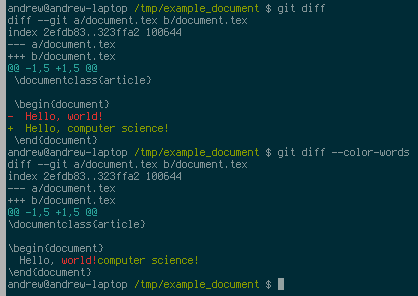
\includegraphics[width=\textwidth]{git_diff}
\end{frame}

\begin{darkframes}
  \begin{frame}{Good packages}
    \begin{itemize}
      \item \texttt{clrscode3e}  -- algorithm typesetting
      \item \texttt{geography} -- paper settings
      \item \texttt{hyperref} -- PDF clickable links
      \item \texttt{minted} -- source code formatting
      \item \texttt{pgf/tikz} -- diagrams
    \end{itemize}
  \end{frame}

  \begin{frame}{Good resources}
    Tutorials and general help
    \begin{itemize}
      \footnotesize
      \item \url{http://andy-roberts.net/writing/latex/}
      \item \url{http://texblog.org}
      \item \texttt{http://uncg.edu/cmp/reu/presentations/Charles Batts - Beamer Tutorial.pdf}
      \item \url{http://tex.stackexchange.com}
    \end{itemize}

    Packages and documentation from \url{http://ctan.org}
  \end{frame}

  \begin{frame}{~}
    \centering
    \vfill
    {\huge Thank You}\\
    andrew.mundy@manchester.ac.uk
    \vfill
  \end{frame}
\end{darkframes}

\end{document}
